\section{Description}
%%%%%%
% Maybe a part here on how to make the junction GC maybe 

\subsection{Elastic medium}
As an introduction of the governing equations, let us describe the elastic medium since the PML is surrounding it. In fact the construction of the PML relies on the same governing equations as the physical medium and share some parameters with it.\\
Let us consider an isotropic homogeneous elastic medium under plane-strain motion and without body forces. The motion in the medium is governed by:
\begin{equation}
\begin{cases}
\sum_{j} \frac{\partial \sigma_{ij}}{\partial x_j} & =  \rho \ddot{u}_i \\
\sigma_{ij} &= \sum_{k,l} C_{ijkl} \epsilon_{kl} \\
\epsilon_{ij} &= \frac{1}{2} \left(\frac{\partial u_{i}}{\partial x_j} + \frac{\partial u_{j}}{\partial x_i} \right)
\end{cases}
\label{eq:2D-motion-elastic}
\end{equation} 
With $u(x,t)$ the displacement, $\epsilon$ the strain, $\sigma$ the stress, $\rho$ the mass density of the medium. $C$ is the material stiffness tensor and its components are expressed in term of the Kronecker delta $\delta_{ij}$:
\begin{equation}
C_{ijkl} = (\kappa-\frac{2}{3}\mu)\delta_{ij}\delta_{kl}+\mu(\delta_{ik}\delta_{jl} + \delta_{il} \delta_{jk})
\end{equation} 
Where $\kappa$ is the bulk modulus and $\mu$ the shear modulus.\\
If we consider an unbounded domain, the system \ref{eq:2D-motion-elastic} admits solutions of the form of P- waves and S-waves. The solutions of P-waves have the following formulation: 
\begin{equation}
u(x,t) = q \exp(-i k_p x . p) \exp(i\omega t)
\label{eq:elastic-sol-p}
\end{equation}
with $k_p = \frac{\omega}{c_p}$ where $\omega$ is the frequency of the wave and $c_p = \sqrt{(\kappa+4\mu/3)/\rho}$ which is the celerity of the P-wave. In the equation \ref{eq:elastic-sol-p} $p$ denotes the unit vector pointing in the direction of propagation of the wave and $q=\pm p$.   
The solution of S-wave form take the following formulation:
\begin{equation}
u(x,t) = q \exp(-i k_s x.p) \exp(i \omega t)
\end{equation}
Where $k_s = \omega / c_s$ and the S-wave speed is $c_s =\sqrt{ \mu/\rho}$ and $q.p =0$.
\subsection{Strong form in frequency domain}
Before describing the governing equations of the two-dimensional PML let us introduce the following notations: $\Omega_{PML}$ will denote the PML domain which is bounded by $\Gamma_{PML} = \Gamma_{PML}^D \cup \Gamma_{PML}^N$. $\Gamma_{PML}^D$ corresponds to the boundary where the Dirichlet condition are applied (imposed displacement). $\Gamma_{PML}^N$ is the boundary where the tractions are applied and represents the boundary of the Neumann conditions. The intersection of these two boundaries defined by the imposed conditions is null: $\Gamma_{PML}^D \cap \Gamma_{PML}^N = \emptyset$. The temporal domain will be denoted by $J = [0,T]$ with $T$ the end time.\\
The classical formulation of PML begins with the introduction of the complex-valued coordinates stretching functions $\lambda_i$. They are used to replace the real coordinates by the complex ones: $x_i \rightarrow \tilde{x}_i: \mathbb{R} \rightarrow \mathbb{C}$.
\begin{equation}
\lambda_i(x_i) = \frac{\partial \tilde{x}_i}{\partial x_i} = 1+f^e_i(x_i)-\frac{i}{b k_s} f^p_i(x_i)
\label{eq:complex-stret-2D}
\end{equation} 
where $b$ is the characteristic length of the problem. $k_s=\omega / c_s$ denotes the wavenumber ($\omega$ is the pulsation and $c_s$ is the celerity of shear waves). $i$ is used to denote the direction $x$ or $y$. $f^p_i$ and $f^e_i$ are the attenuation functions for respectively propagating and evanescent waves. They are written as a polynomial of order $n$. 
\begin{equation}
f^\alpha_i = a_\alpha \left(\frac{x_i - x_0}{L_{p,i}}  \right), x_i \in [x0,x0+d] \\
\label{eq:attenuation-functions}
\end{equation}
% Little explanation of what is the effect of the coordinate stretching function ? 
The tunable property of the PML relies mainly on the formulation of the attenuation functions. The value of the coefficients of attenuation $a_p$, $a_e$, the order of the polynomial $n$, and the size of the PML $L_p$ can be defined by the user. As we will see in the section concerning the numerical results, these parameters need to be chosen carefully and depending on the problem to obtain the "best" result possible. The concept of "best result" depends on the expectations of the user. Accuracy versus performance is a deep-seated problem for all numerical simulations. The perfectly matched layer does not get out of this rule. In order to choose the value of these coefficients, we can use the reflection coefficient for an incident pressure wave given by \cite{Basu2004}:
\begin{equation}
R_{pp} = \frac{cos(\theta+\theta_s)}{cos(\theta-\theta_s)} \exp\left[-2\frac{c_s}{c_p}F_1(L_p)cos(\theta)\right]
\label{eq:Rpp} 
\end{equation} 
Where $c_p$ stands for the velocity of P-waves. The incident P-wave is characterised by $\theta$, its angle of incidence and $\theta_s$, its reflective angle after being reflected at the end of the PML. $F_1$ corresponds to the integral over the PML of the attenuation function for propagating waves: $F_1(L_p) = \int_{s=0}^{L_p} f^p(s) ds = \frac{\beta_0 L_p}{n+1}$. Thus, the attenuation coefficients can be expressed in function of the reflection coefficient:
\begin{equation}
a_\alpha = \ln\left(\frac{cos(\theta+\theta_s)}{R_{pp}cos(\theta-\theta_s)} \right) \frac{c_p}{c_s} \frac{n+1}{L_p cos(\theta)}
\label{eq:alpha_kucu}
\end{equation} 
If we consider that the incident wave has an angle of $\theta = \theta_s = 0$ therefore the value of the coeffecient has the form:
\begin{equation}
a_\alpha = \ln\left(\frac{1}{R_{pp}} \right) \frac{c_p}{c_s} \frac{n+1}{L_p cos(\theta)}
\end{equation}
\par Using the complex-valued coordinates stretching functions \ref{eq:complex-stret-2D}, the strong form of the equations of motion for the PML in the frequency domain is defined by:
\begin{equation}
\begin{cases}
\sum_{j} \frac{1}{\lambda_j(x_j)} \frac{\partial \sigma_{ij}}{\partial x_j} & = - \omega^2 \rho u_i \\
\sigma_{ij} &= \sum_{k,l} C_{ijkl} \epsilon_{kl} \\
\epsilon_{ij} &= \frac{1}{2} \left(\frac{1}{\lambda_j(x_j)} \frac{\partial u_{i}}{\partial x_j} + \frac{1}{\lambda_i(x_i)} \frac{\partial u_{j}}{\partial x_i} \right)
\end{cases}
\label{eq:2D-PML-freq}
\end{equation} 
Where $C_{ijkl}$ are the components of the elastic constitutive tensor. In fact the system \ref{eq:2D-PML-freq} defines a perfectly matched medium (PMM) and the elastic medium is just a specific case of PMM with $\lambda_j(x_j) = 1$, $\forall x \in \Omega_{PML}$. If we imagine a PML, surrounding an elastic medium, as in the figure \ref{fig:scheme-layers}, we have to define for the PML $\lambda_j(x_j) = 1$ for $\forall x \in \Gamma_{PML}$ at the interface between the two-subdomains. \\
The system of equations \ref{eq:2D-PML-freq} assumes harmonic time-dependence of the displacement, stress and strain. Therefore, its solution can be written as $u(x,t) = \overline{u}(x,t)exp(i \omega t)$. If the stretching functions have the formulation \ref{eq:complex-stret-2D} then the system \ref{eq:2D-PML-freq} has solutions of the form: 
\begin{equation}
\overline{u}(x) = \exp[-\frac{c_s}{c_p}\sum_i F_i(x_i)p_i ] q  \exp(i k_p x . p)
\end{equation}
with $q = \pm p$, and
\begin{equation}
\overline{u}(x) = \exp [ -\sum_i F_i(x_i)p_i ] q  \exp(- i k_s x . p)
\end{equation}
with $q.p=0$ and $F_i(x_i) = \int_0^{x_i} f_i(\xi) d\xi$.\\
Therefore the solution admitted in the PML corresponds to the solution of the system \ref{eq:2D-motion-elastic} but with an imposed spatial attenuation. 
The attenuation contained in the term $\exp[ - F_i p_i ]$ for the direction $i$ is independent of the frequency if the direction of propagation is. 


\begin{figure}[H]
\centering
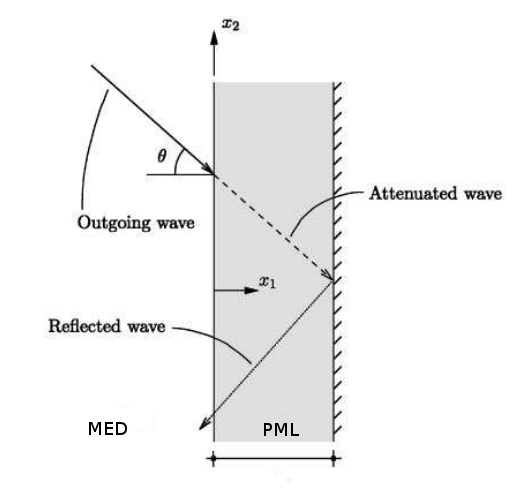
\includegraphics[scale=0.5]{images/scheme-layers.png}
\caption{Scheme of the propagation of a wave within the elastic medium (on the left) and the PML (on the right)}
\label{fig:scheme-layers}
\end{figure} 
\subsection{Strong form in time domain}
\par The strong form of the PML in the temporal domain can be obtained by inverse Fourier transform of each equation of \ref{eq:2D-PML-freq}. Indeed the introduction of the complex-valued coordinates stretching functions makes the application of this inverse easier. In the following equation the number of lines below a tensor will specify its order. 
%% Explanation on how to obtain these equations (for final version) maybe in appendice
\begin{equation}
\begin{cases}
div(\doubleunderline{\sigma}\tilde{F}^e + \doubleunderline{\Sigma}\tilde{F}^p) = \rho f_m \underline{\ddot{u}} + \rho \frac{c_s}{b} f_c \underline{\dot{u}} + \frac{\mu}{b^2}f_k \underline{u}, & \text{In } \Omega_{PML} \times J\\
\doubleunderline{\sigma} =  C : \doubleunderline{\epsilon} , & \text{In } \Omega_{PML} \times J\\
F^{eT} \doubleunderline{\dot{\epsilon}}F^e + F^{pT}\underline{\epsilon}F^e + F^{eT}\doubleunderline{\epsilon}F^p + F^{pT} \doubleunderline{E} F^p = ...\\
\frac{1}{2}(\nabla \underline{\dot{u}}^T F^e + F^{eT} \nabla \underline{\dot{u}})+\frac{1}{2}(\nabla \underline{u}^T F^p + F^{pT} \nabla \underline{u}), & \text{In } \Omega_{PML} \times J\\
\end{cases}
\label{eq:2D-PML-strong-timeD}
\end{equation}
submitted to the homogeneous boundary conditions:
\begin{equation}
\begin{cases}
\underline{u}=0,& \text{on } \Gamma_{PML}^D\\
(\doubleunderline{\sigma}\tilde{F}^e + \doubleunderline{\Sigma}\tilde{F}^p).n , & \text{on } \Gamma_{PML}^N 
\end{cases}
\label{eq:conditions-lim}
\end{equation}
Let us now summarize the form of the different matrices $F^e,F^p,\tilde{F}^e$ and $\tilde{F}^p$ of the above equations.
\begin{equation}
F^e = \begin{bmatrix}
1+f^e_1(x1)&0\\0&1+f^e_2(x2)
\end{bmatrix}, F^p = \begin{bmatrix}
\frac{c_s}{b}f^p_1(x1)&0\\0&\frac{c_s}{b}f^p_2(x2) 
\end{bmatrix} 
\end{equation}
\begin{equation}
\tilde{F}^e = \begin{bmatrix}
1+f^e_2(x2)&0\\0&1+f^e_1(x1)
\end{bmatrix}, \tilde{F}^p = \begin{bmatrix}
\frac{c_s}{b}f^p_2(x2)&0\\0&\frac{c_s}{b}f^p_1(x1) 
\end{bmatrix} 
\end{equation}
Let us now focus on the first equation of \ref{eq:2D-PML-strong-timeD}, the functions $f_m$, $f_c$ and $f_k$ depend on the attenuation functions:
\begin{equation}
\begin{cases}
f_m = (1+f^e_1(x1))(1+f^e_2(x2))\\
f_c = (1+f^e_1(x1))f^p_2(x2) + (1+f^e_2(x2))f^p_1(x1)\\
f_k = f^p_1(x_1)f^p_2(x_2)
\end{cases}
\end{equation}
The next elements to define, which appear in the first and the third equations of \ref{eq:2D-PML-strong-timeD} are the integral of the stress and the strain.
\begin{equation}
\doubleunderline{\Sigma} = \int^t_0 \doubleunderline{\sigma} dt, \doubleunderline{E} = \int^t_0 \doubleunderline{\epsilon} dt
\end{equation} 
\subsection{Displacement-based weak form}
Let us introduce the test function $\underline{v}$ belonging to an admissible space of solution $V$. Premultiplying the first equation of the strong form \ref{eq:2D-PML-strong-timeD} by $\underline{v}$ and integrating over the PML domain gives :
\begin{align}
\int_{\Omega_{PML}} \underline{v}.div(\doubleunderline{\sigma}\tilde{F}^e + \doubleunderline{\Sigma}\tilde{F}^p) d\Omega_{PML} & = \int_{\Omega_{PML}} \rho f_m \underline{v}.\underline{\ddot{u}} d\Omega_{PML} + ... \nonumber\\
&  \int_{\Omega_{PML}} \rho \frac{c_s}{b} f_c \underline{v}.\underline{\dot{u}} d\Omega_{PML} +  \int_{\Omega_{PML}} \frac{\mu}{b^2}f_k \underline{v}. \underline{u}  d\Omega_{PML},  \text{In } \Omega_{PML} \times J 
\label{eq:weak-form-motion}
\end{align}
Using the Gauss divergence theorem and integration per parts gives:

\begin{multline}
\int_{\Gamma_{PML}} \underline{v} .\left(\doubleunderline{\sigma}\tilde{F}^e + \doubleunderline{\Sigma}\tilde{F}^p \right).\underline{n} d\Gamma_{PML}  = \int_{\Omega_{PML}} \rho f_m \underline{\ddot{u}} . \underline{v} d\Omega_{PML} + ... \nonumber\\
\int_{\Omega_{PML}} \rho \frac{c_s}{b} f_c \underline{\dot{u}} . \underline{v} d\Omega_{PML} +  \int_{\Omega_{PML}} \frac{\mu}{b^2}f_k \underline{u} . \underline{v} d\Omega_{PML} +\int_{\Omega_{PML}} \doubleunderline{\tilde{\epsilon}}^e : \doubleunderline{\sigma} d\Omega_{PML} + \int_{\Omega_{PML}} \doubleunderline{\tilde{\epsilon}}^p : \doubleunderline{\Sigma} d\Omega_{PML},  \text{In } \Omega_{PML} \times J
\end{multline}
$\underline{n}$ is the vector normal to the boundary of the PML $\Gamma_{PML}$. The tensors $\doubleunderline{\tilde{\epsilon}}^p$ and $\doubleunderline{\tilde{\epsilon}}^e$ depend on the attenuation functions:
\begin{equation}
\begin{cases}
\doubleunderline{\tilde{\epsilon}}^e = \frac{1}{2}\left(\nabla \underline{v} \tilde{F}^e + \tilde{F}^{eT} \nabla \underline{v}^T  \right) \\
\doubleunderline{\tilde{\epsilon}}^p = \frac{1}{2}\left(\nabla \underline{v} \tilde{F}^p + \tilde{F}^{pT} \nabla \underline{v}^T  \right)
\end{cases}
\label{eq:weak-first-eq}
\end{equation}
Using the weak form of the equation of motion within the PML in the temporal domain \ref{eq:weak-form-motion} we can define the mass, damping and stiffness matrices:
\begin{equation}
m^{e} = \int_{\Omega_e} \rho f_m N_I N_J d\Omega_e I_d
\label{eq:2Dpml-elem-mass}
\end{equation}
\begin{equation}
 c^{e} = \int_{\Omega_e} \rho f_c \frac{c_s}{b} N_I N_J d\Omega_e I_d
 \label{eq:2Dpml-elem-damp}
\end{equation}
\begin{equation}
  k^{e} = \int_{\Omega_e} \frac{\mu}{b^2} f_k N_I N_J d\Omega_e I_d 
  \label{eq:2Dpml-elem-stiff}
\end{equation}
In the above equation $N_I$ is the nodal shape function for node $I$.
Let us introduce a notation for the internal forces term: 
\begin{equation}
p^e = \int_{\Omega_{PML}} \doubleunderline{\tilde{\epsilon}}^e : \doubleunderline{\sigma} d\Omega_{PML} + \int_{\Omega_{PML}} \doubleunderline{\tilde{\epsilon}}^p : \doubleunderline{\Sigma} d\Omega_{PML}
\end{equation}
In order to modify this term we need to make a temporal discretization.
\subsection{Complete discrete form}
Before describing the complete discrete equations of two-dimensional PML featuring the discretization in space and time, we need to introduce the following notation. The hat notation above an element will specify that the tensor is written in Voigt notation. For example $\hat{\sigma} = \begin{pmatrix}
\sigma_{11} \\
\sigma_{22} \\
\sigma_{12}
\end{pmatrix}$ 
Thus, using a simple temporal discretization with $dt=t_{n+1} - t_n$ we can rewrite the internal forces at time $t_{n+1}$ as:
\begin{equation}
p_{n+1}^e = \int_{\Omega_e} \tilde{B}^{eT} \hat{\sigma}_{n+1} d\Omega_e + \int_{\Omega_e}\tilde{B}^{pT} \hat{\Sigma}_{n+1} d\Omega_e
\label{eq:intern-forces-discrete}
\end{equation} 
The two matrices $\tilde{B}^{p}$ and $\tilde{B}^{e}$ in \ref{eq:intern-forces-discrete} depend on the nodal shape functions and the attenuation functions. They are expressed in term of their nodal submatrices as:
\begin{equation}
\tilde{B}^e_I = \begin{bmatrix}
\tilde{N}^e_{I1}&0\\0&\tilde{N}^e_{I2}\\\tilde{N}^e_{I2}&\tilde{N}^e_{I1}
\end{bmatrix}, \tilde{B}^p_I = \begin{bmatrix}
\tilde{N}^p_{I1}&0\\0&\tilde{N}^p_{I2}\\\tilde{N}^p_{I2}&\tilde{N}^p_{I1}
\end{bmatrix}
\end{equation} 
with 
\begin{equation}
\tilde{N}^e_{Ii} = \tilde{F}^e_{ji}N_{I,j}, \tilde{N}^p_{Ii} = \tilde{F}^p_{ji}N_{I,j}
\end{equation}
And
\begin{equation}
\tilde{B}^T = \tilde{B}^{eT}+dt \tilde{B}^{pT}
\end{equation}
\begin{equation}
B^\epsilon_I = \begin{bmatrix}
F^\epsilon_{11}N^I_{I1}&F^\epsilon_{21}N^I_{I1}\\
F^\epsilon_{12}N^I_{I2}&F^\epsilon_{22}N^I_{I2}\\
F^\epsilon_{11}N^I_{I2}+F^\epsilon_{12}N^I_{I1}& F^\epsilon_{21}N^I_{I2}+F^\epsilon_{22}N^I_{I1}
\end{bmatrix}
\end{equation}
Some assumptions have to be made to perform time stepping. To evaluate the integral of the stress or strain at the next time step we will assume that:
\begin{equation}
\begin{cases}
\hat{\Sigma}_{n+1} &= \hat{\Sigma}_n + dt \hat{\sigma}_{n+1} \\
\hat{E}_{n+1} &= \hat{E}_n + dt \hat{\epsilon}_{n+1}
\end{cases}
\end{equation}
Thus using this assumption, the internal forces term can be rewrite as:
\begin{equation}
p_{n+1}^e = \int_{\Omega_e} \tilde{B}^{T} \hat{\sigma}_{n+1} d\Omega_e + \int_{\Omega_e}\tilde{B}^{pT} \hat{\Sigma}_{n} d\Omega_e
\end{equation}
where
\begin{equation}
\tilde{B}^{T} = \tilde{B}^{eT} + dt \tilde{B}^{pT}
\end{equation}
An additional assumption has to be made to evaluate the derivative of the strain:
\begin{equation}
\dot{\epsilon}_{n+1} = \frac{\epsilon_{n+1}-\epsilon_n}{dt}
\end{equation} 
This correspond to the first order approxiation due to Taylor's theorem.
Using this assumption in the third equation of \ref{eq:2D-PML-strong-timeD} the expression of the strain for the next time step can be obtained.
\begin{equation}
\hat{\epsilon}_{n+1} = \frac{1}{dt}\left(B^\epsilon \dot{U}_{n+1} + B^Q U_{n+1} + \frac{1}{dt} \hat{F}^\epsilon \hat{\epsilon}_n - \hat{F}^Q \hat{E}_n\right)
\label{eq:strain-n+1}
\end{equation} 
The matrices $B^\epsilon$, $B^Q$, $\hat{F}^\epsilon$ and $\hat{F}^Q$ depend on the attenuation and the nodal shape functions. The are defined by their nodal submatrices as:
\begin{equation}
B^\epsilon_I = \begin{bmatrix}
F^\epsilon_{11}N^I_{I1}&F^\epsilon_{21}N^I_{I1}\\
F^\epsilon_{12}N^I_{I2}&F^\epsilon_{22}N^I_{I2}\\
F^\epsilon_{11}N^I_{I2}+F^\epsilon_{12}N^I_{I1}& F^\epsilon_{21}N^I_{I2}+F^\epsilon_{22}N^I_{I1}
\end{bmatrix}
\end{equation}
with
\begin{equation}
N^I_{Ii} = F^I_{ij}N_{I,j}
\end{equation}
\begin{equation}
F^I = \left[ F^p+\frac{F^e}{dt} \right]^{-1}, F^\epsilon = F^eF^I, F^Q=F^pF^I
\end{equation}
and
\begin{equation}
\hat{F}^\epsilon_I = \begin{bmatrix}
(F^\epsilon_{11})^2&(F^\epsilon_{21})^2& F^\epsilon_{11}F^\epsilon_{21}\\
(F^\epsilon_{12})^2&(F^\epsilon_{22})^2&F^\epsilon_{12}F^\epsilon_{22}\\
2F^\epsilon_{11}F^\epsilon_{12}&2 F^\epsilon_{21}F^\epsilon_{22}& F^\epsilon_{11}F^\epsilon_{22}+F^\epsilon_{12}F^\epsilon_{21}
\end{bmatrix}
\end{equation}
To obtain the relations for $B^Q$ and $\hat{F}^Q$ the only thing to replace is the superscript $\epsilon$ by $Q$. 
\par The stress $\hat{sigma}_{n+}$ is computed using the second equation of \ref{eq:2D-PML-strong-timeD} involving the elastic constitutive tensor $C$. Thus the internal forces term can be expressed in function of the strain and not the stress.
\begin{equation}
p_{n+1}^e = \int_{\Omega_e} \tilde{B}^{T} D \hat{\epsilon}_{n+1} d\Omega_e + \int_{\Omega_e}\tilde{B}^{pT} \hat{\Sigma}_{n} d\Omega_e
\end{equation} 
and using the relation \ref{eq:strain-n+1} this expression can be rewrite as:
\begin{align}
p_{n+1}^e &= \int_{\Omega_e} \tilde{B}^{T} D \left[\frac{1}{dt}\left(B^\epsilon \dot{U}_{n+1} + B^Q U_{n+1} + \frac{1}{dt} \hat{F}^\epsilon \hat{\epsilon}_n - \hat{F}^Q \hat{E}_n\right)  \right] d\Omega_e + \int_{\Omega_e}\tilde{B}^{pT} \hat{\Sigma}_{n} d\Omega_e \\
&= \tilde{c}^e \dot{U}^e_{n+1} + \tilde{k}^e U^e_{n+1} + P(\hat{\epsilon}_n,\hat{E}_n,\hat{\Sigma}_n)
\end{align} 
where 
\begin{equation}
P(\hat{\epsilon}_n,\hat{E}_n,\hat{\Sigma}_n) = \int_{\Omega_e} \tilde{B}^T \frac{D}{dt} \left[\frac{1}{dt}\hat{F}^{\epsilon} \hat{\epsilon} - \hat{F}^Q \hat{E}_n \right] + \tilde{B}^p \hat{\Sigma}_n d\Omega_e
\label{eq:pseudo-intern}
\end{equation}
and 
\begin{equation}
\tilde{c}^{e} = \frac{1}{dt} \int_{\Omega_e} \tilde{B}^T D B^\epsilon d\Omega_e
\label{eq:2Dpml-elem-effdamp}
\end{equation}
\begin{equation}
\tilde{k}^{e} = \frac{1}{dt} \int_{\Omega_e} \tilde{B}^T D B^Q d\Omega_e
\label{eq:2Dpml-elem-effstiff}
\end{equation}
Under the plane-strain assumption the material constitutive matrix is expressed as:
\begin{equation}
\begin{pmatrix}
K+\frac{4}{3}\mu_L& K-\frac{2}{3}\mu_L&0\\
K-\frac{2}{3}\mu_L&K+\frac{4}{3}\mu_L&0\\
0&0&\mu_L
\end{pmatrix}
\end{equation}
Therefore using the above equation we can rewrite \ref{eq:weak-first-eq} as:
\begin{equation}
M\ddot{U}_{n+1} + \left(C+\tilde{C}\right)\dot{U}_{n+1} + \left(K+\tilde{K}\right)U_{n+1} + P(\hat{\epsilon}_n,\hat{E}_n,\hat{\Sigma}_n) = F_{ext}
\label{eq:2Dpml-discrete-motion}
\end{equation}
Where $M$,$C$ and $K$ are respectively the mass, damping and stiffness matrices resulting from the assembly of their element matrices \ref{eq:2Dpml-elem-mass}, \ref{eq:2Dpml-elem-damp} and \ref{eq:2Dpml-elem-stiff}. The matrices $\tilde{K}$ and $\tilde{C}$ derive from the assembly procedure of their element matrices \ref{eq:2Dpml-elem-effstiff} and \ref{eq:2Dpml-elem-effdamp}. $P(\hat{\epsilon}_n,\hat{E}_n,\hat{\Sigma}_n)$ is given by the equation \ref{eq:pseudo-intern} and is known at the beginning of the time step since it depends only on components of the previous time. 
\subsection{Time integration scheme}
The complete discrete equations obtained in the previous part acn be integrated using the Newmark-$\beta$ scheme. The classical Newmark approximation formulas are expressed in acceleration form:
\begin{equation}
\begin{cases}
U_{n+1} = U_{n,p} + \beta dt^2 \ddot{U}_{n+1} \\
\dot{U}_{n+1} = \dot{U}_{n,p} + \gamma dt \ddot{U}_{n+1}
\end{cases}
\label{eq:newmark1}
\end{equation}
where the predictors $U_{n,p}$ and $\dot{U}_{n,p}$ have the form:
\begin{equation}
\begin{cases}
U_{n,p} = U_n + dt \dot{U}_n + dt^2 \left(\frac{1}{2} -\beta  \right)\ddot{U}_n \\
\dot{U_{n,p}} = \dot{U}_n + dt (1-\gamma)\ddot{U}_n
\end{cases}
\label{eq:newmark2}
\end{equation}
Substituing the equations \ref{eq:newmark1} and \ref{eq:newmark2} into the discrete form of the equation of motion \ref{eq:2Dpml-discrete-motion} the acceleration at time $t_{n+1}$ can be obtained.
\begin{equation}
\tilde{M}\ddot{U}_{n+1} = F_{ext} - \left(C+\tilde{C}\right)\dot{U}_{n,p} - \left(K+\tilde{K}\right)U_{n,p} - P(\hat{\epsilon}_n,\hat{E}_n,\hat{\Sigma}_n)
\end{equation}
where 
\begin{equation}
\tilde{M} = M + \gamma dt \left(C+\tilde{C}\right) + \beta dt^2 \left(K+\tilde{K}\right)
\end{equation}
This matrix need to be inverted, this will be done before beginning the time stepping since all the matrices constituing it remain constant through the time stepping. Two schemes will be used in the following of this report:
\begin{itemize}
\item Implicit Newmark scheme: with $\gamma = 1/2$ and $\beta = 1/4$.
\item Explicit Newmark scheme: with $\gamma = 1/2$ and $\beta = 0$.
\end{itemize} 
The properties of each schemes will be investigated in the next section concerning the stability and the last part will highlight the differences in term of performance and accuracy.









 





